\documentclass[a4paper,12pt,russian]{extreport}
\usepackage[utf8]{inputenc}
\usepackage[T2A]{fontenc}
\usepackage[russian]{babel}
\usepackage{graphicx}
\usepackage{amsmath}

% далее две строки отвечающие за т.н. "полуторный интервал"
%\usepackage[nodisplayskipstretch]{setspace}
%\onehalfspacing
%\parskip 1.5ex % paragraph spacing

\usepackage{geometry}
\geometry{left=3cm}
\geometry{right=1.5cm}
\geometry{top=2cm}
\geometry{bottom=2cm}

%\renewcommand{\rmdefault}{ftm} 
%\frenchspacing

\usepackage{authblk}
\title{Отчет по лабораторной работе №3 «Решение СЛАУ прямыми методами. Теория возмущений» Вариант~№22}
\author{Левицкий Валентин А-13-22}
\affil{НИУ «МЭИ»}
\date{\today}
\begin{document}

\maketitle
\section*{Задача 3.1}
Реализовать решение СЛАУ с помощью LU разложения и LU разложения по схеме частичного выбора. Решить систему небольшой размерности с возмущенной матрицей обоими методами, оценить погрешность и сравнить с теоретической оценкой. Проанализировать поведение  методов с ростом числа уравнений.

$A_{ij} = \arctan(0.1 (10i + j + 1)).$

\subsection*{Решение}
Напишим функцию создания матрицы размера m:
\begin{verbatim}
def init_matr(m):
    matr = np.zeros((m, m))
    for i in range(m):
        for j in range(m):
            matr[i][j] = np.arctan(0.1 * (10 * i + j + 1))
    return matr
\end{verbatim}

1. Реализуем метод решения СЛАУ с помощью LU разложения по схеме единственного деления, модифицирующий исходную матрицу A.
\begin{verbatim}
def LU(A) -> np.array:
    lu = A.copy()
    for i in range(1, A.shape[0]):
        for j in range(0, i):
            mu = lu[i, j] / lu [j, j]
            mask = np.ones_like(lu[j, :])
            mask[:j] = 0
            # print(lu[j, :] * mask)
            lu[i, :] -= mu * (lu[j, :] * mask)
            lu[i, j] = mu
    return lu

def solve(A, b):
    lu = LU(A)
    l = np.tril(lu, -1) + np.eye(lu.shape[0])
    u = np.triu(lu)
    # print(l)
    # print(u)
    y = np.linalg.inv(l).dot(b)
    x = np.linalg.inv(u).dot(y)
    # return l, u
    return x
\end{verbatim}

Убедимся в работоспособности метода:
\begin{verbatim}
solve(A, b)

array([[22. , 22. , 22.00000001, 22. , 22. ]])
\end{verbatim}

2. Реализуем метод решения СЛАУ с помощью LU разложения по схеме частичного выбора в виде двух функций, одна из которых возвращает две матрицы – L и U, не модифицируя A, а вторая функция решает систему.
\begin{verbatim}
def Mimod(A, k, is_l):
    mi = np.eye(*A.shape)
    P = np.eye(*A.shape)
    mx = k + np.argmax(np.abs(A[k:, k]))
    P[[k, mx]] = P[[mx, k]]
    A = P.dot(A)
    for i in range(k + 1, A.shape[1]):
        mi[i, k] = A[i, k] / A[k, k]
        if not is_l:
            mi[i, k] *= -1
    return mi, P

def LUmod(A):
    U = A.copy()
    L = np.eye(*A.shape)
    M = np.eye(*A.shape)
    for j in range(0, A.shape[1] - 1):
        mi, pi = Mimod(U, j, False)
        mii, pii = Mimod(U, j, True)
        U = mi.dot(pi).dot(U)
        L = L.dot(pii).dot(mii)
    return L, U

def solvemod(A, b):
    L, U = LUmod(A)
    y = np.linalg.inv(L) @ b
    x = np.linalg.inv(U) @ y
    return x
\end{verbatim}

Убедимся в работоспособности метода:
\begin{verbatim}
solve(A, b)

array([[22. , 21.99999999, 22.00000002, 21.99999998, 22. ]])
\end{verbatim}

3. Решим систему  $A^*x = b$, размера 5 x 5, двумя методами. $A^*$ зададим как $A$ и к одному элементу прибавим $10^{-3}$  
\begin{verbatim}
A_star  = A.copy()
A_star[3, 3] += 0.001
x1 = solve(A_star, b)
x2 = solvemod(A_star, b)
\end{verbatim}

4. Вычислим погрешности и сравним с теоретической оценкой.
\begin{verbatim}
Dx1 = np.linalg.norm(x_root - x1)
Dx2 = np.linalg.norm(x_root - x2)
DA = np.linalg.norm(A - A_star)
dx1 = Dx1 / np.linalg.norm(x_root)
dx2 = Dx2 / np.linalg.norm(x_root)
dA = DA / np.linalg.norm(A)
condA = np.linalg.norm(A) * np.linalg.norm(np.linalg.inv(A))
d_hat = condA * DA
print(f'{dx1 = }')
print(f'{dx2 = }')
print(f'Теоретическая оценка: {d_hat}')


dx1 = 0.8568133536857635
dx2 = 0.8568133536692295
Теоретическая оценка: 56493.659253590085
\end{verbatim}

Погрешность решений полученых обоими методами находится в пределах теоретической оценки.

5. Решим систему обоими методами для матриц большей размерности. Построим на одном графике погрешности обоих методов как функций, зависящих от $n$.

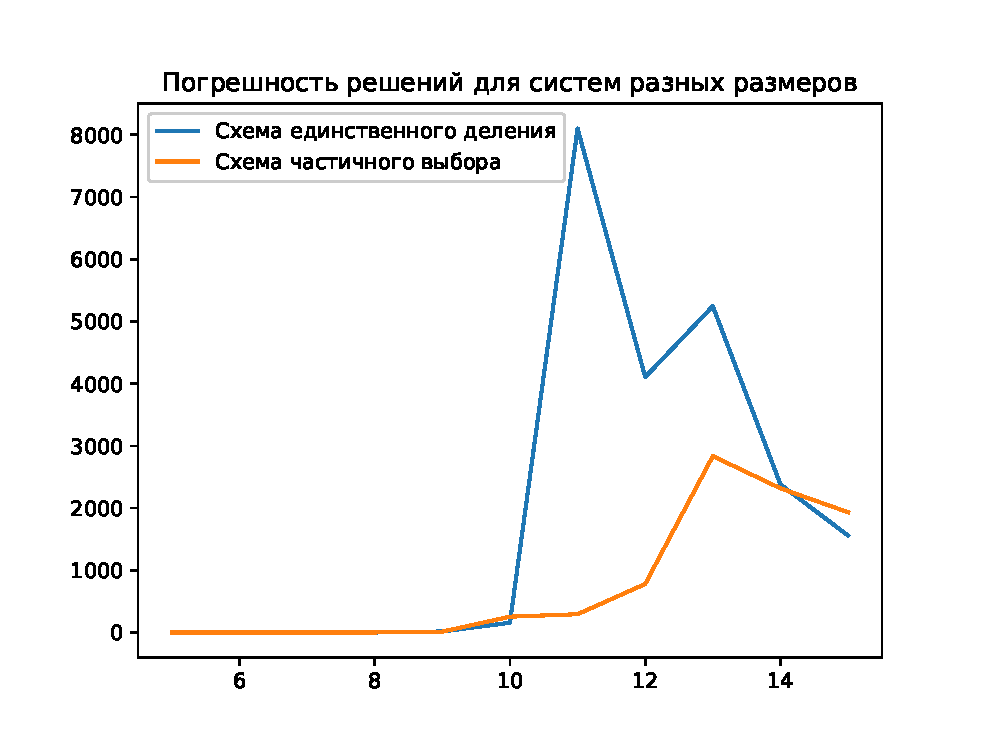
\includegraphics[width=15cm]{311.eps}

Из графиков видно, что погрешность прямых методов возрастает с размерами системы, при этом метод частичного выбора дает более точный результат.

\section*{Задача 3.2}
Дана разреженная матрица A. Найти число обусловленности матрицы.

\subsection*{Решение}
1. Зададим матрицу А согласно схеме из приложения: все ненулевые элементы матрицы равны $N$ ( номеру варианта), элементы главной диагонали равны  $N*m+m/N$,  $m$ - размерность матрицы.


\begin{verbatim}
A = np.eye(20, 20)
A[:8,:4] = N
A[8:14, 4:8] = N
A[14:, :8] = N
for i in range(8, m-1):
    A[i, i+1:] = N
for i in range(m):
    A[i, i] = (N*m + m/N)
\end{verbatim}

2.Разработаем и реализуем алгоритм решения системы с данной матрицей $А$ прямым методом с учетом нулевых элементов.
\begin{verbatim}
def zerofy(B, n):
    """Зануляет элеметны строки n, находящиеся под главной диагональю."""
    for i in range(0, n):
        mu = B[n, i] / B[i, i]
        B[n, :] -= mu * B[i, :]
    return B

def simplify(A, b):
    """Приводит разреженную матрицу А к двухдиагональному виду"""
    B = np.concatenate((A, b), axis = 1)
    for i in range(1, 8):
        B[i-1, :] -= B[i, :]
    for i in range(9, 20):
        B[i-1, :] -= B[i, :]
    B = zerofy(B, 7)
    B = zerofy(B, 13)
    B = zerofy(B, 19)
    return B[:, :-1], B[:, -1]

def backward(A, b):
    """Обратный ход для двухдиагональной матрицы"""
    x = np.zeros_like(b)
    x[-1] = b[-1] / A[-1, -1]
    for i in range(b.size-2, -1, -1):
        x[i] = (b[i] - A[i, i+1] * x[i+1]) / A[i, i]
    return x

def fast_solve(A, b):
    return backward(*simplify(A, b))
\end{verbatim}

\includegraphics[width=15cm]{matr.png}

Выполним проверку, взяв вектор $x$, состоящий из одинаковых элементов $33$:
\begin{verbatim}
x_root = np.ones((20, 1)) * 33
b = A.dot(x_root)
fast_solve(A, b)

array([33., 33., 33., 33., 33., 33., 33., 33., 33., 33., 33.,
        33., 33., 33., 33., 33., 33., 33., 33., 33.])
\end{verbatim}

3. Напишим алгоритм для поиска обратной матрицы, основанный на решении уравнений $Ax^j=E^j$, где $E^j$ - столбцы единичной матрицы, проверим работоспособность:
\begin{verbatim}
def inv(A):
    ans = np.eye(*A.shape)
    for j in range(A.shape[1]):
        ans[:, j] = fast_solve(A, ans[:, j].reshape(A.shape[0], 1))
    return ans
\end{verbatim}

Проверим работоспособность алгоритма:

\begin{verbatim}
np.max(np.abs(inv(A).dot(A) - np.eye(20, 20)))

2.220446049250313e-16
\end{verbatim}


4. Найдем число обусловленности матрицы, используя евклидову норму:
\begin{verbatim}
condA = np.linalg.norm(A) * np.linalg.norm(inv(A))
condA

20.37275136439184
\end{verbatim}

5. Вывод

1. Данная матрица является хорошо обусловленной т.к. $cond A < 100$;

2. Трудоемкость метода составила:
   - 57m вычитаний, 3m умножений - функция simplify;

   - 3m вычитаний и умножений - функция backward;

   - Итого ~63m операций, т.е. сложность алгоритма - линейная.

\section*{Задача 3.3}
Дана система уравнений $Ax = b$ c матрицей $A$ из задачи 3.2 и вектором $b:\ b_i = |N - 25| + 5$, где N - номер варианта. Решить систему методом Якоби с точностью $\varepsilon = 10^{-10}$.

\subsection*{Решение}
1. Составим программу преобразования системы $Ax = b$ к виду $x = Bx + c$.

\begin{verbatim}
def Jacobi(A, b):
    '''Перобразует СЛАУ Ax=b к виду x = Bx + c.'''
    B = np.zeros_like(A)
    c = np.zeros_like(b)
    for i in range(A.shape[1]):
        B[i, :] = -A[i, :] / A[i, i]
        B[i, i] = 0
        c[i,0] = b[i,0] / A[i, i]
    return B, c
\end{verbatim}

Убедимся, что выполнено достаточное условие сходимости метода: $||B|| < 1$
\begin{verbatim}
B, c = Jacobi(A, b)
np.linalg.norm(B)

0.6428766787355629
\end{verbatim}

2. Составим программу метода простых итераций с подсчетом нормы вектора невязки на каждой итерации.
\begin{verbatim}
def MPI(A, b, eps):
    B, c = Jacobi(A, b)
    x0 = c
    x1 = B.dot(x0) + c
    iters = 1
    r_n = []
    k = (1 - inf_norm(B)) / inf_norm(B)
    while inf_norm(x1 - x0) > k * eps:
        r_n.append(euclid_norm(A.dot(x1) - b))
        x0 = x1
        x1 = B.dot(x1) + c
        iters +=1
    print("Выполнено итераций: ", iters)
    return x1, np.array(r_n)
\end{verbatim}

Убедимся, что выполнено достаточное условие сходимости метода: $||B|| < 1$.
\begin{verbatim}
B, c = Jacobi(A, b)
np.linalg.norm(B)

0.6428766787355629
\end{verbatim}

Составим программу метода простых итераций с подсчетом нормы вектора невязки на каждой итерации.
\begin{verbatim}
def MPI(A, b, eps):
    B, c = Jacobi(A, b)
    x0 = c
    x1 = B.dot(x0) + c
    iters = 1
    r_n = []
    k = (1 - inf_norm(B)) / inf_norm(B)
    while inf_norm(x1 - x0) > k * eps:
        r_n.append(euclid_norm(A.dot(x1) - b))
        x0 = x1
        x1 = B.dot(x1) + c
        iters +=1
    print("Выполнено итераций: ", iters)
    return x1, np.array(r_n)
\end{verbatim}

Найдем решение задачи с заданной точностью.

\begin{verbatim}
x, r_n = MPI(A, b, eps)

Выполнено итераций:  13
\end{verbatim}

Подставим найденое решение в исходное уравнение и убедимся в корректности метода:
\begin{verbatim}
A.dot(x).T

array([[8., 8., 8., 8., 8., 8., 8., 8., 8., 8., 8., 8., 8., 8., 8., 8.,
        8., 8., 8., 8.]])
\end{verbatim}

Нормы векторов невязки по итерациям:

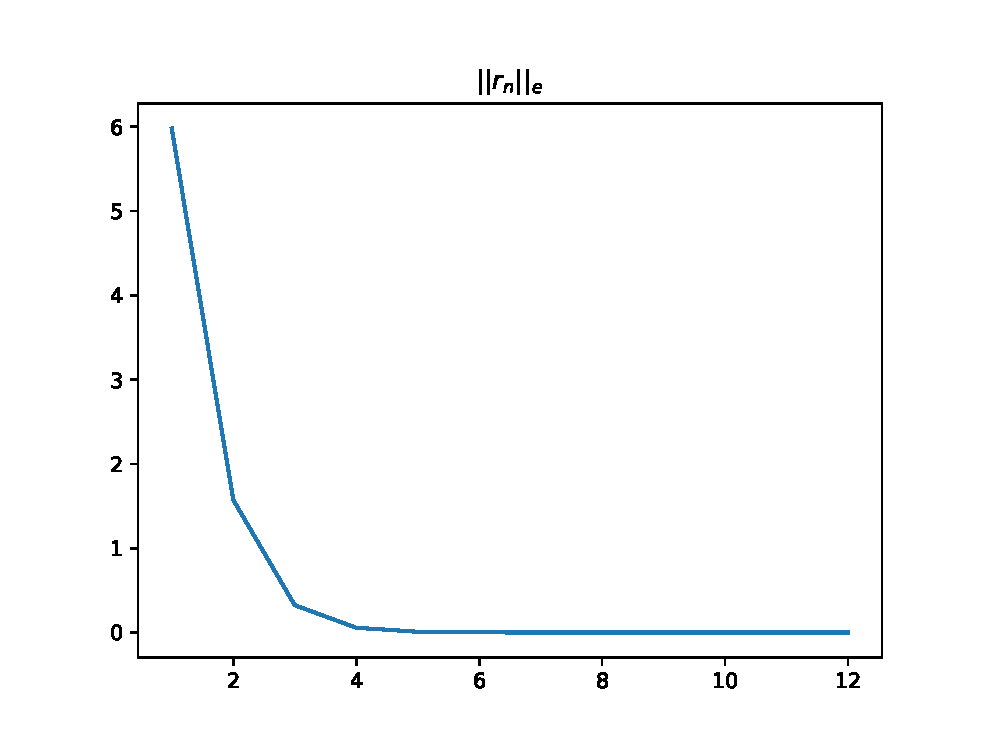
\includegraphics[width=15cm]{fig331.eps}

\end{document}
